\chapter{Blocklyでの用語}\label{chap:blocklyWord}

本研究はBlocklyをベースにして行うため,次節以降には,Blocklyのユーザインタフェース固有の用語が出現する.
それに先立ち,主要となる用語と概念を本節で共有する.

\begin{description}
 \item[{\tt コネクタ:}]
ブロックとブロックを接続する切り欠きを表すオブジェクト(図\ref{fig:connector}).
コネクタには4種類あり,
値の入力を受け取る入力コネクタ,
値の出力を表す出力コネクタ,
上向きまたは下向きに付くステートメントコネクタがある.
図\ref{fig:connector}の右にあるブロックが示すように,ブロックの移動時には,
ユーザがブロックを接続しやすいように,近くにある接続可能なコネクタがハイライトされる.

 \item[{\tt フライアウトメニュー:}]
ブロックを新しく生成するためのメニュー(図\ref{fig:workspace}).
定義されたブロックが並んでおり,ドラッグをすると新しいブロックをそのまま得ることができる.

 \item[{\tt ワークスペース:}]
ブロックの組み立てやドラッグ移動などを自由に行うことのできる空間のこと.
空間ごとの座標系や拡大縮小の制御,発火イベントの管理などを担っている.
ワークスペースはブロックと同様に,SVGエレメントとしても実態を持っており,
ブロックを表すSVGエレメントはこのワークスペースの空間を表したSVGグループの中に内包されている.
各ブロックは必ず1つのワークスペースに属している.

 \item[{\tt メインワークスペース:}]
フライアウトメニューから生成したブロックを自由に組み立てることのできる
一番根本にあるワークスペースのこと(図\ref{fig:workspace}).

\end{description}

\begin{figure}[t]
 \centering
 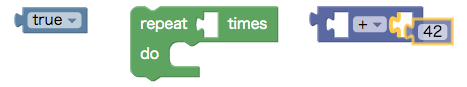
\includegraphics[keepaspectratio, scale=0.5]{img/connector.png}
 \caption{Blockly上でのブロックの例.
各ブロックに外向きについている切り欠きの部分がコネクタである.\label{fig:connector}}
 \centering
 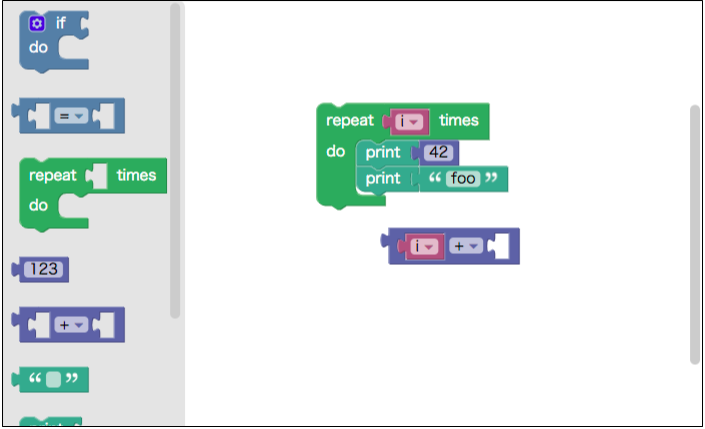
\includegraphics[keepaspectratio, scale=0.3]{img/blocklyWorkspace.png}
 \caption{Blocklyでのフライアウトメニュー,メインワークスペースを示したもの.
 左側の背景色が灰色の部分がフライアウトメニューであり,
 右側の背景色が白色の部分がメインワークスペースである.\label{fig:workspace}}
\end{figure}
